% !TEX root = ../main.tex
\section{Segmentación y visualización con paletas de color}

    El resultado de un proceso de segmentación o análisis a menudo es una imagen monocanal (una máscara, un mapa de probabilidad, un mapa de distancia). La forma en que visualizamos este resultado es crítica para su correcta interpretación. Podemos utilizar estas herramientas durante el proceso de análisis de una imagen.
    \subsection{Consigna}
        \begin{itemize}[leftmargin=*]
            \item Elegir una imagen a color con bajo contraste.
            \item Umbralizar un objeto de interés en el espacio que crea adecuado (pero sin binarizarlo, es decir, manteniendo los valores continuos).
            \item Ecualizar el histograma.
            \item Visualizar esta imagen monocanal resultante utilizando al menos cuatro paletas de color diferentes, de modo de resaltar detalles sutiles antes no perceptibles
            \item Determinar la paleta apropiada para representar lo que se quiera destacar.
            \item Evaluar la precisión de la segmentación lograda.
        \end{itemize}

    \subsection{Análisis de imagen elegida:}
        Para este análisis se optó por utilizar la misma imagen de bajo contraste utilizada en el punto  de anterior de ecualización de contraste (\textbf{Figura \ref{fig:ej3_casos}}). En primera instancia se determinó si la imagen seleccionada presenta contraste bajo, sabiendo que el contraste es la relación entre las zonas más brillantes y más oscuras de una imagen, mediante un histograma de la luminancia, tanto de los canales RGB como también de la combinación ponderada de dichos canales (escala de grises) (\textbf{Figura \ref{fig:ej4_analisis_imagen}}).
         
        \begin{figure}[H] \centering
            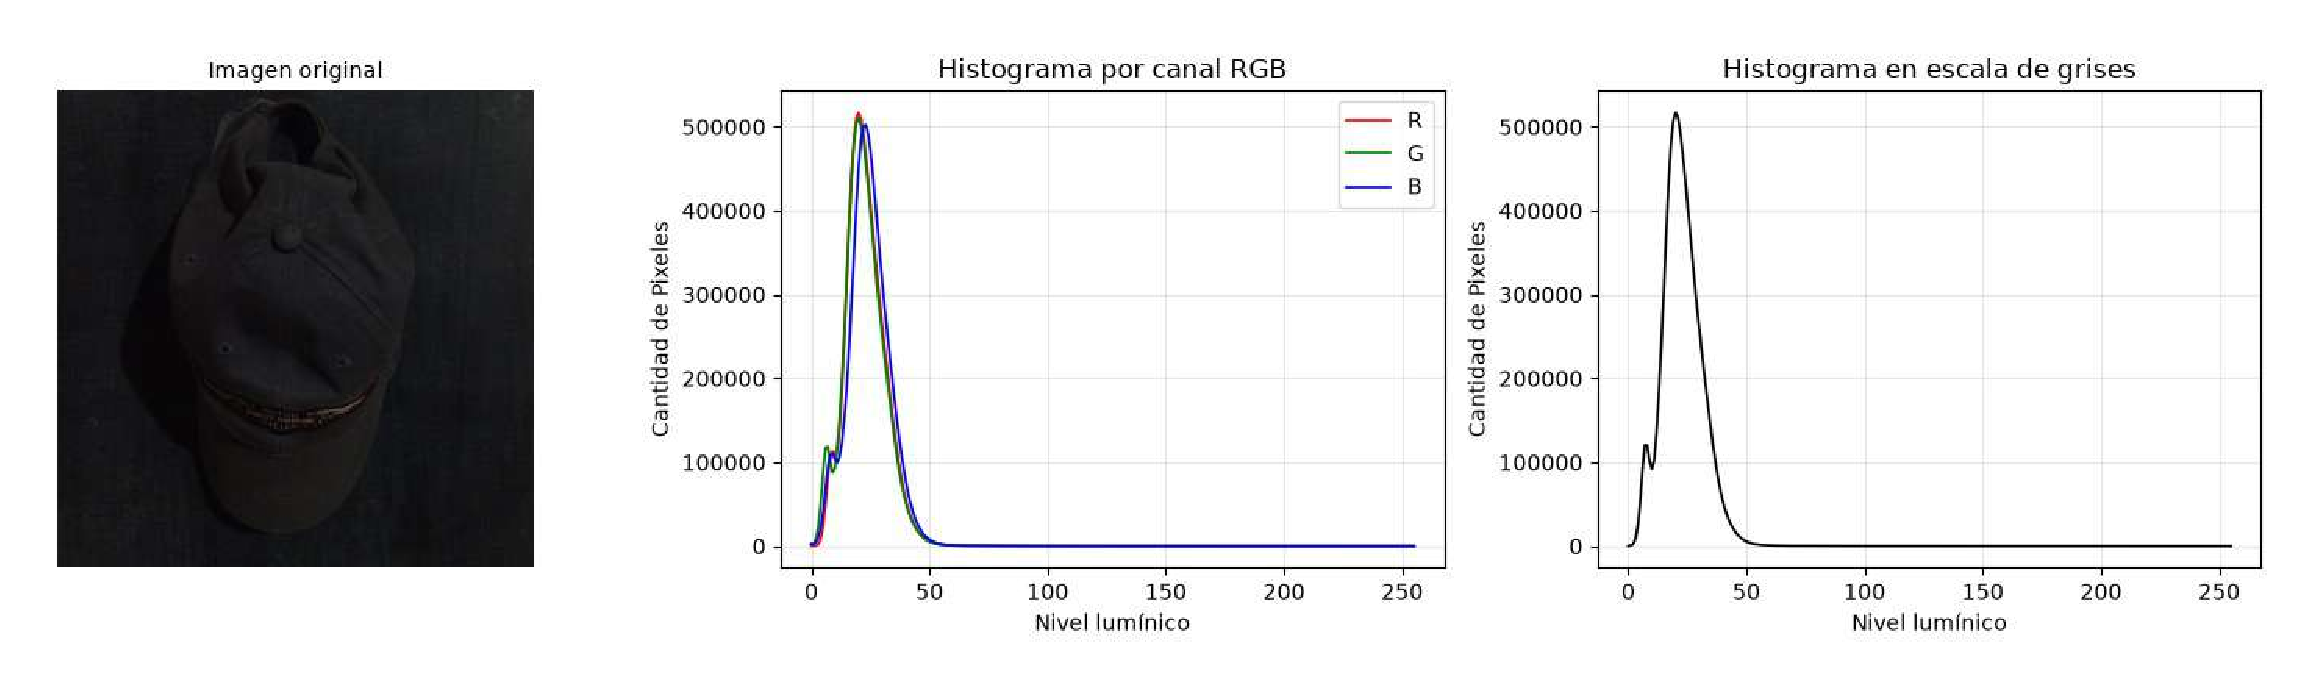
\includegraphics[width=\linewidth]{img/ejercicio4/imagen_analizada.pdf}
            \caption{Imágenes utilizadas para el análisis.}
            \label{fig:ej4_analisis_imagen}
        \end{figure}

        Además, para no depender de una apreciación puramente visual por parte de los histogramas se planteó un análisis analítico de los valores como la desviación estándar, media lumínica y contraste RMS (\textbf{Tabla \ref{tab:ej4_metricas_contraste}}).

        \begingroup \setstretch{1.1}
            \begin{table}[H] \centering
                \begin{tblr}{
                    colspec = {lcX}, width = \linewidth, rowsep = 2pt, colsep = 6pt, hlines, vlines,
                    cells = {valign = m}, row{1} = {bg = gray!15, font = \bfseries, halign = c}
                }
                    Métrica & Valor & Qué mide \\
                    Media lumínica ($\mu$) & 22.76 & Brillo global promedio de la imagen. \\
                    Desviación estándar ($\sigma$) & 8.45 & Dispersión de las intensidades (contraste absoluto). \\
                    Contraste RMS & 0.371 & Variación tonal relativa al brillo medio ($\sigma/\mu$). \\
                \end{tblr}
                \caption{Métricas de contraste y luminancia de la imagen analizada.}
                \label{tab:ej4_metricas_contraste}
            \end{table}
        \endgroup

        Los valores analíticos obtenidos demuestran que la imagen seleccionada presenta un contraste bajo,
        ya que la desviación estándar de la luminocidad ($\sigma=8.45$) es de solo 8 a 9 niveles luminicos lo cual es muy pequeño comparado con el rango de intensidades posibles (0 a 255). El contraste RMS confirma que la dispersión es pequeña comparada con el brillo medio, y el rango efectivo p1–p99 (que representa el 98\% de la informacion real de la imagen) ocupa solo una pequeña fracción (12\%) del histograma, concentrándose en la zona oscura del mismo.


        Primeramente, antes de la umbralización, se determinó como espacio seleccionado al espacio de escala de grises ya que en el espacio RGB, la información de la iluminación y el matiz están fusionadas y una simple sombra altera los tres canales a la vez. Sin embargo en este espacio, al ser una media ponderada de los canales RGB, sufre menos de estos problemas ya que aísla la información de reflectancia lumínica de la imagen, desacoplándola del color.


        Posterior a esto se realizó la umbralización manteniendo los valores continuos ya que al binarizar aplanamos la imagen, convirtiendo todos los píxeles válidos a 255 (blanco) y destruyendo la información de textura, volumen y gradientes originales. Se eligió el método ``A Zero Invertido'' con un umbral fijo $T$ obtenido a partir de aplicar Otsu sobre el canal de escala de grises redondeado al múltiplo de 5. Esta técnica se seleccionó porque permite conservar el rango oscuro de la imagen (donde se encuentra el objeto de interés) con sus valores originales, apagando las zonas claras. Los resultados comparativos de las diferentes variantes no binarias, como el corte en seco de ``A Zero'' y una transición de atenuación con una ``Rampa suave'', se detallan en la \textbf{Figura \ref{fig:ej4_umbralizacion}}.

        \begin{figure}[H] \centering
            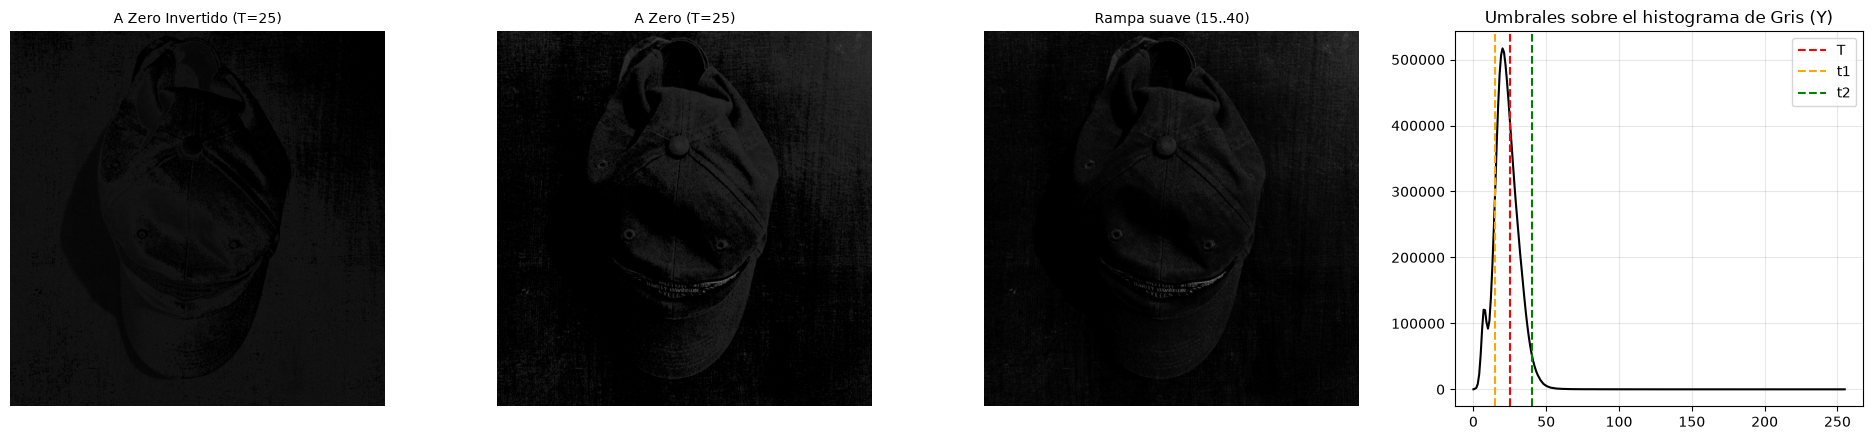
\includegraphics[width=\linewidth]{img/ejercicio4/umbralizacion.png}
            \caption{Comparación de umbralizaciones sin binarizar sobre el canal de escala de grises.}
            \label{fig:ej4_umbralizacion}
        \end{figure}

        A continuación, se aplicó una ecualización global al resultado monocanal obtenido en el paso anterior, preservando la máscara de ceros original. De esta forma, se reubican las intensidades con un único mapeo monótono en toda la imagen y se logra el resultado visualizado en la \textbf{Figura \ref{fig:ej4_ecualizacion}}. Se descartó el estiramiento y la ecualización adaptativa (CLAHE) dado que el primero no ecualiza el histograma sino que lo recorta, y el segundo aplica mapeos distintos por región, ocasionando que se observen menos detalles de textura y relieve en la gorra y fondo.

        \begin{figure}[H] \centering
            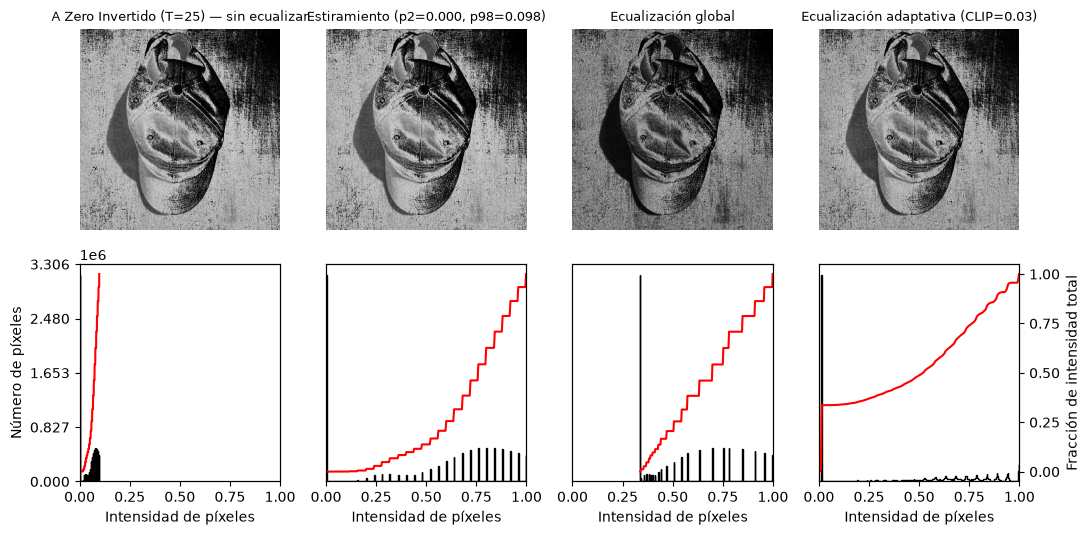
\includegraphics[width=\linewidth]{img/ejercicio4/ecualizacion.png}
            \caption{Comparación de técnicas de ecualización sobre la imagen umbralizada.}
            \label{fig:ej4_ecualizacion}
        \end{figure}

        Para visualizar mejor los resultados, se representó la imagen monocanal umbralizada y ecualizada utilizando distintas paletas de colores: gray, viridis, plasma, hot y jet (\textbf{Figura \ref{fig:ej4_paletas}}). Se mantuvo el mismo rango de valores en todas ellas para poder comparar en igualdad de condiciones. Se observó que la paleta viridis proporciona un gradiente secuencial y perceptualmente uniforme; la paleta gray provee una buena referencia acromática, mientras que plasma y hot enfatizan mayores rangos cromáticos e intuitivos (como la asociación de calor a brillo).

        \begin{figure}[H] \centering
            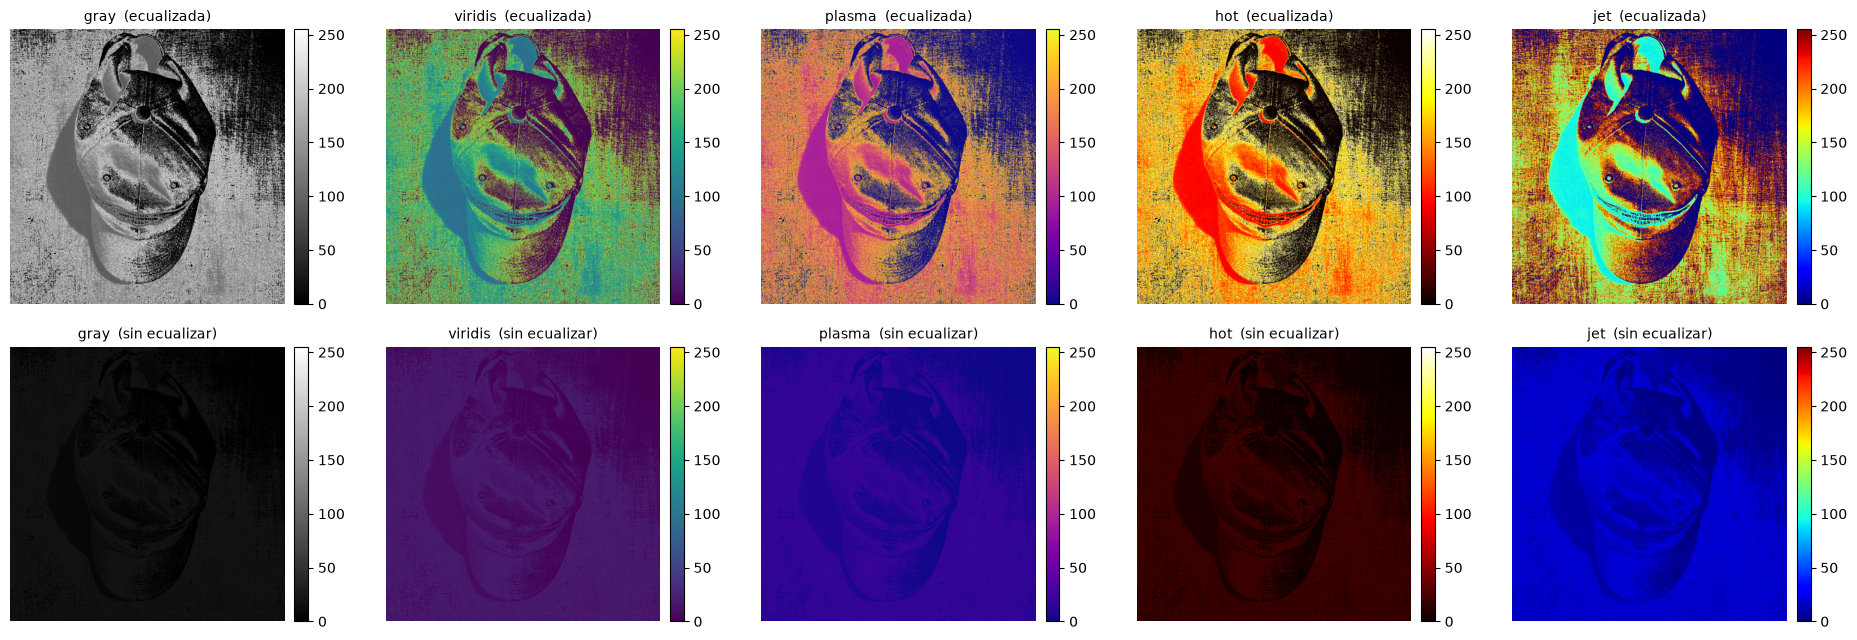
\includegraphics[width=\linewidth]{img/ejercicio4/paletas.png}
            \caption{Visualización de la imagen segmentada con distintas paletas, con y sin ecualizar.}
            \label{fig:ej4_paletas}
        \end{figure}


        Como se pudo observar en la \textbf{Figura \ref{fig:ej4_paletas}}, las paletas plasma y hot  son las que permiten visualizar mejor los detalles sutiles de la imagen como la textura del fondo (tiza mal borrada del pizarrón usado de fondo) y a su vez resalta de manera intuitivamente visible zonas con diferente profundidad (o relieve), dado que proporciona un gradiente secuencial y perceptualmente uniforme.

    \subsection{Preguntas y análisis}

        \begin{itemize}[leftmargin=*]
            \item Comparar la visualización con `gray' y con `viridis'. ¿En cuál resulta más fácil distinguir las variaciones sutiles en los datos?

            Resulta más fácil en viridis. Esto se debe a que gray mapea el dato a luminancia pura, y nuestro sistema visual tiene limitaciones para distinguir diferencias pequeñas de brillo de manera fina. En cambio, viridis varía tono y brillo a la vez, permitiendo notar cambios sutiles como los patrones de la tiza en el pizarrón y algunos relieves causado por los dobleces de la gorra.
            
            \item Para algunas paletas, ¿se observa la aparición de `bandas' o `contornos' que no parecen corresponderse con una transición suave en los datos? Explicar por qué ocurre esto (ver propiedades de la paleta, graficar su perfil de luminancia por ejemplo).

            Sí, se observan fuertemente contornos falsos y bandas en paletas como jet (y transiciones poco suaves en regiones de hot o plasma). Ocurre debido a que su perfil de luminancia no es monótono (caso jet) ni lineal, provocando que variaciones graduales de los datos se traduzcan en diferencias bruscas de color que el sistema visual percibe de manera exagerada.


            Respecto a la aparición de bandas, se procedió a graficar el perfil de luminancia para estas paletas (\textbf{Figura \ref{fig:ej4_luminancia}}). De este análisis se desprende que las ``bandas'' perceptuales aparecen por fluctuaciones no lineales o no monótonas en la luminancia de la paleta.

            \begin{figure}[H] \centering
                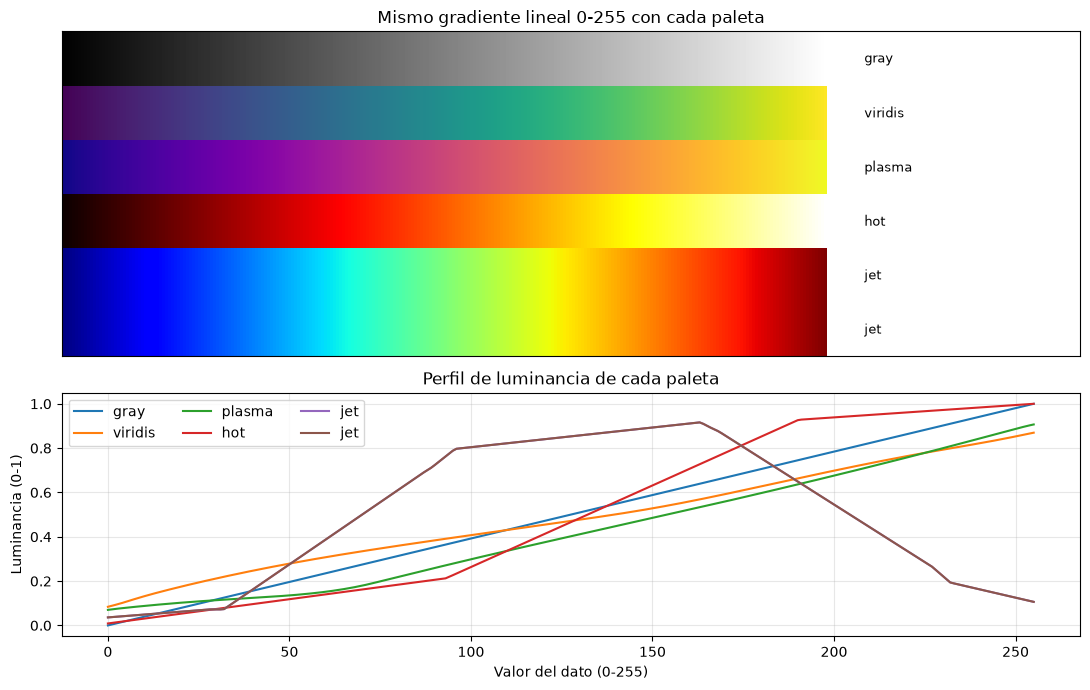
\includegraphics[width=\linewidth]{img/ejercicio4/luminancia.png}
                \caption{Análisis del perfil de luminancia para distintas paletas.}
                \label{fig:ej4_luminancia}
            \end{figure}

            \item ¿Cuál de las paletas probadas comunica la información de la imagen (monocanal) de manera más clara y honesta? Justificar elección. ¿Es objetivo el criterio o depende de la percepción de cada uno?
            
            La paleta viridis (a diferencia de jet) comunica de manera más clara y honesta al tratar datos secuenciales. Su perfil de luminancia es monótono y casi lineal, garantizando que el color cambie parejo con el dato. Este criterio es en parte objetivo (ya que la monotonicidad y uniformidad son cuantificables y medibles) pero también subjetivo, porque depende del observador y de las caracteristicas que se desee destacar.

            \item Luego de la segmentación inicial y ecualización del resultado, ¿resulta factible umbralizar detalles pequeños que en un inicio no lo eran?
            
            Sí, resulta factible. La ecualización redistribuye las intensidades de modo que detalles que antes ocupaban un rango muy estrecho (por ejemplo, las marcas de tiza en el pizarrón o los pliegues de la gorra) pasan a ocupar un rango más amplio dentro del histograma. Al estar más separados del fondo, estos detalles pueden aislarse con un segundo umbral que originalmente no los habría distinguido. No obstante, la mejora no es uniforme: los detalles ubicados en zonas del histograma donde la ecualización comprime niveles (pendiente menor a 1) pueden seguir siendo difíciles de separar.

            \item Una mala elección de paleta de colores, ¿puede llevar a un análisis erróneo de la información presente en la imagen?
            
            Sí, rotundamente. Una paleta categórica o no monótona puede inventar estructuras inexistentes, introducir bandas o contornos falsos (creando artefactos), o simplemente ocultar información sutil bajo gradientes que no son perceptualmente lineales y no estan alineados con la forma en que el sistema visual humano procesa la luz.

            \item ¿Puedo segmentar sobre un canal de color determinado? ¿Y aplicar la máscara a todos los canales de la imagen?
            
            Sí, la segmentación suele realizarse sobre un único canal (como el de escala de grises o aquel con mayor contraste para el objeto de interés) porque simplifica la umbralización a un problema unidimensional. El resultado es una matriz lógica o máscara bidimensional (de ceros y unos). Como los tres canales de la imagen a color (RGB) comparten exactamente las mismas coordenadas espaciales, esta máscara se puede aplicar multiplicándola punto a punto por cada canal individualmente. De esta forma, se aíslan los píxeles de interés recuperando su color original sin que la crominancia afecte las reglas de segmentación.

        \end{itemize}
